% ---------------------------------------------------------------------------------------
\chapter{Resultados sobre el banco de im\'agenes}\label{appA}

En este apendice incluimos los resultados obtenidos sobre el banco de im\'agenes, para los distintos experimentos y otras figuras de interes. 


\begin{figure}[H]
    \centering
    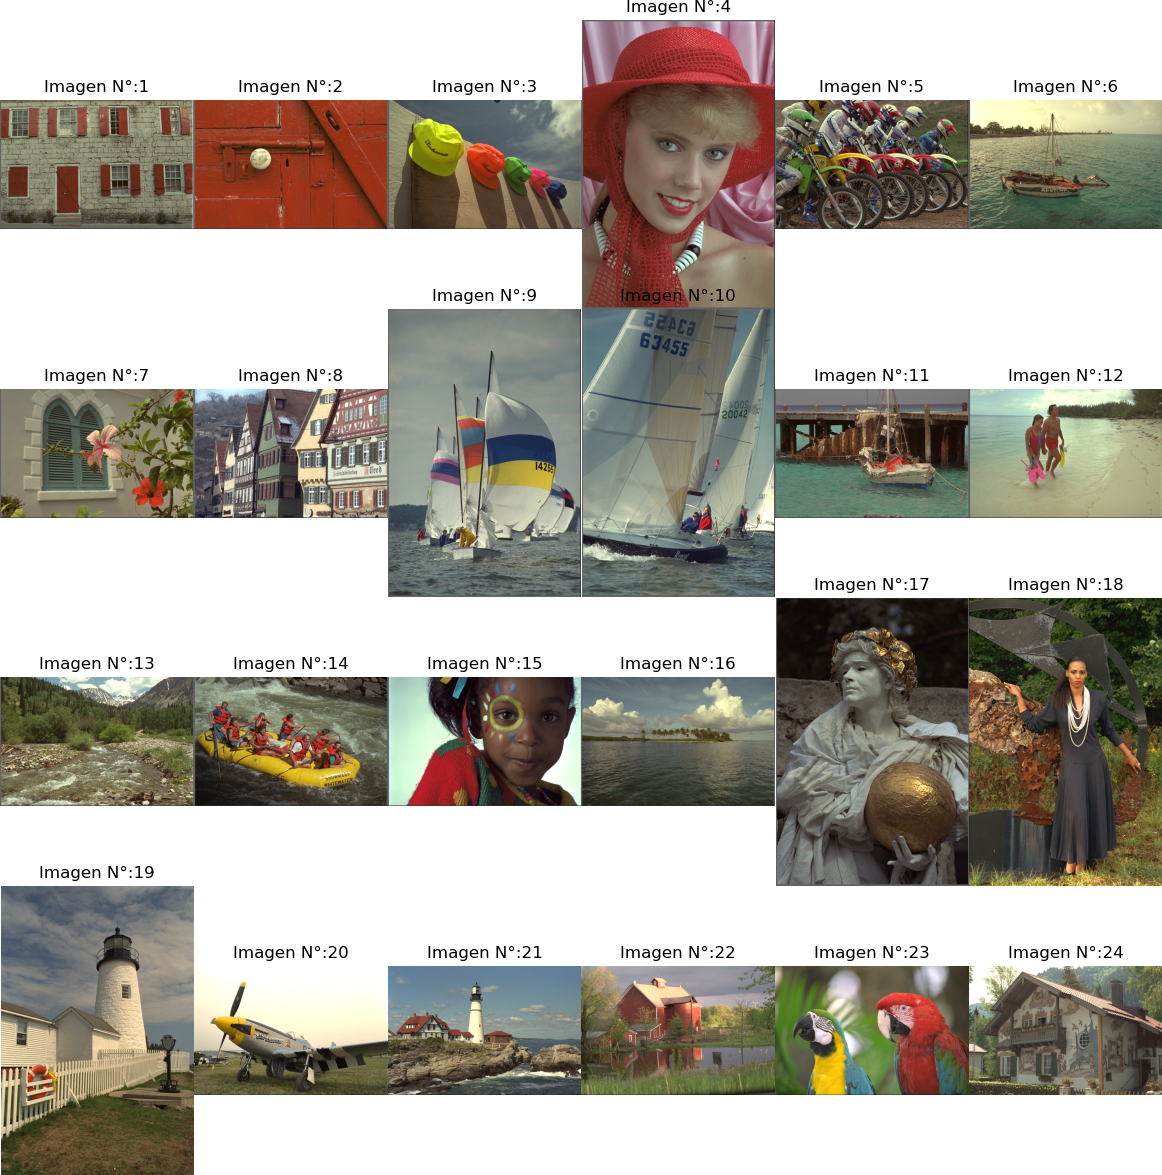
\includegraphics[width=0.7\textwidth]{figuras/all_images_in_order.png}
    \caption{imagenes en el orden original del Banco.}
\end{figure}


\begin{figure}
    \centering
    \includegraphics[width=0.6\textwidth]{figuras/img_hist_all.png}
    \caption{Imagen original e histomgrama para todas imagenes del banco, en orden.}
\end{figure}

\begin{figure}
    \centering
    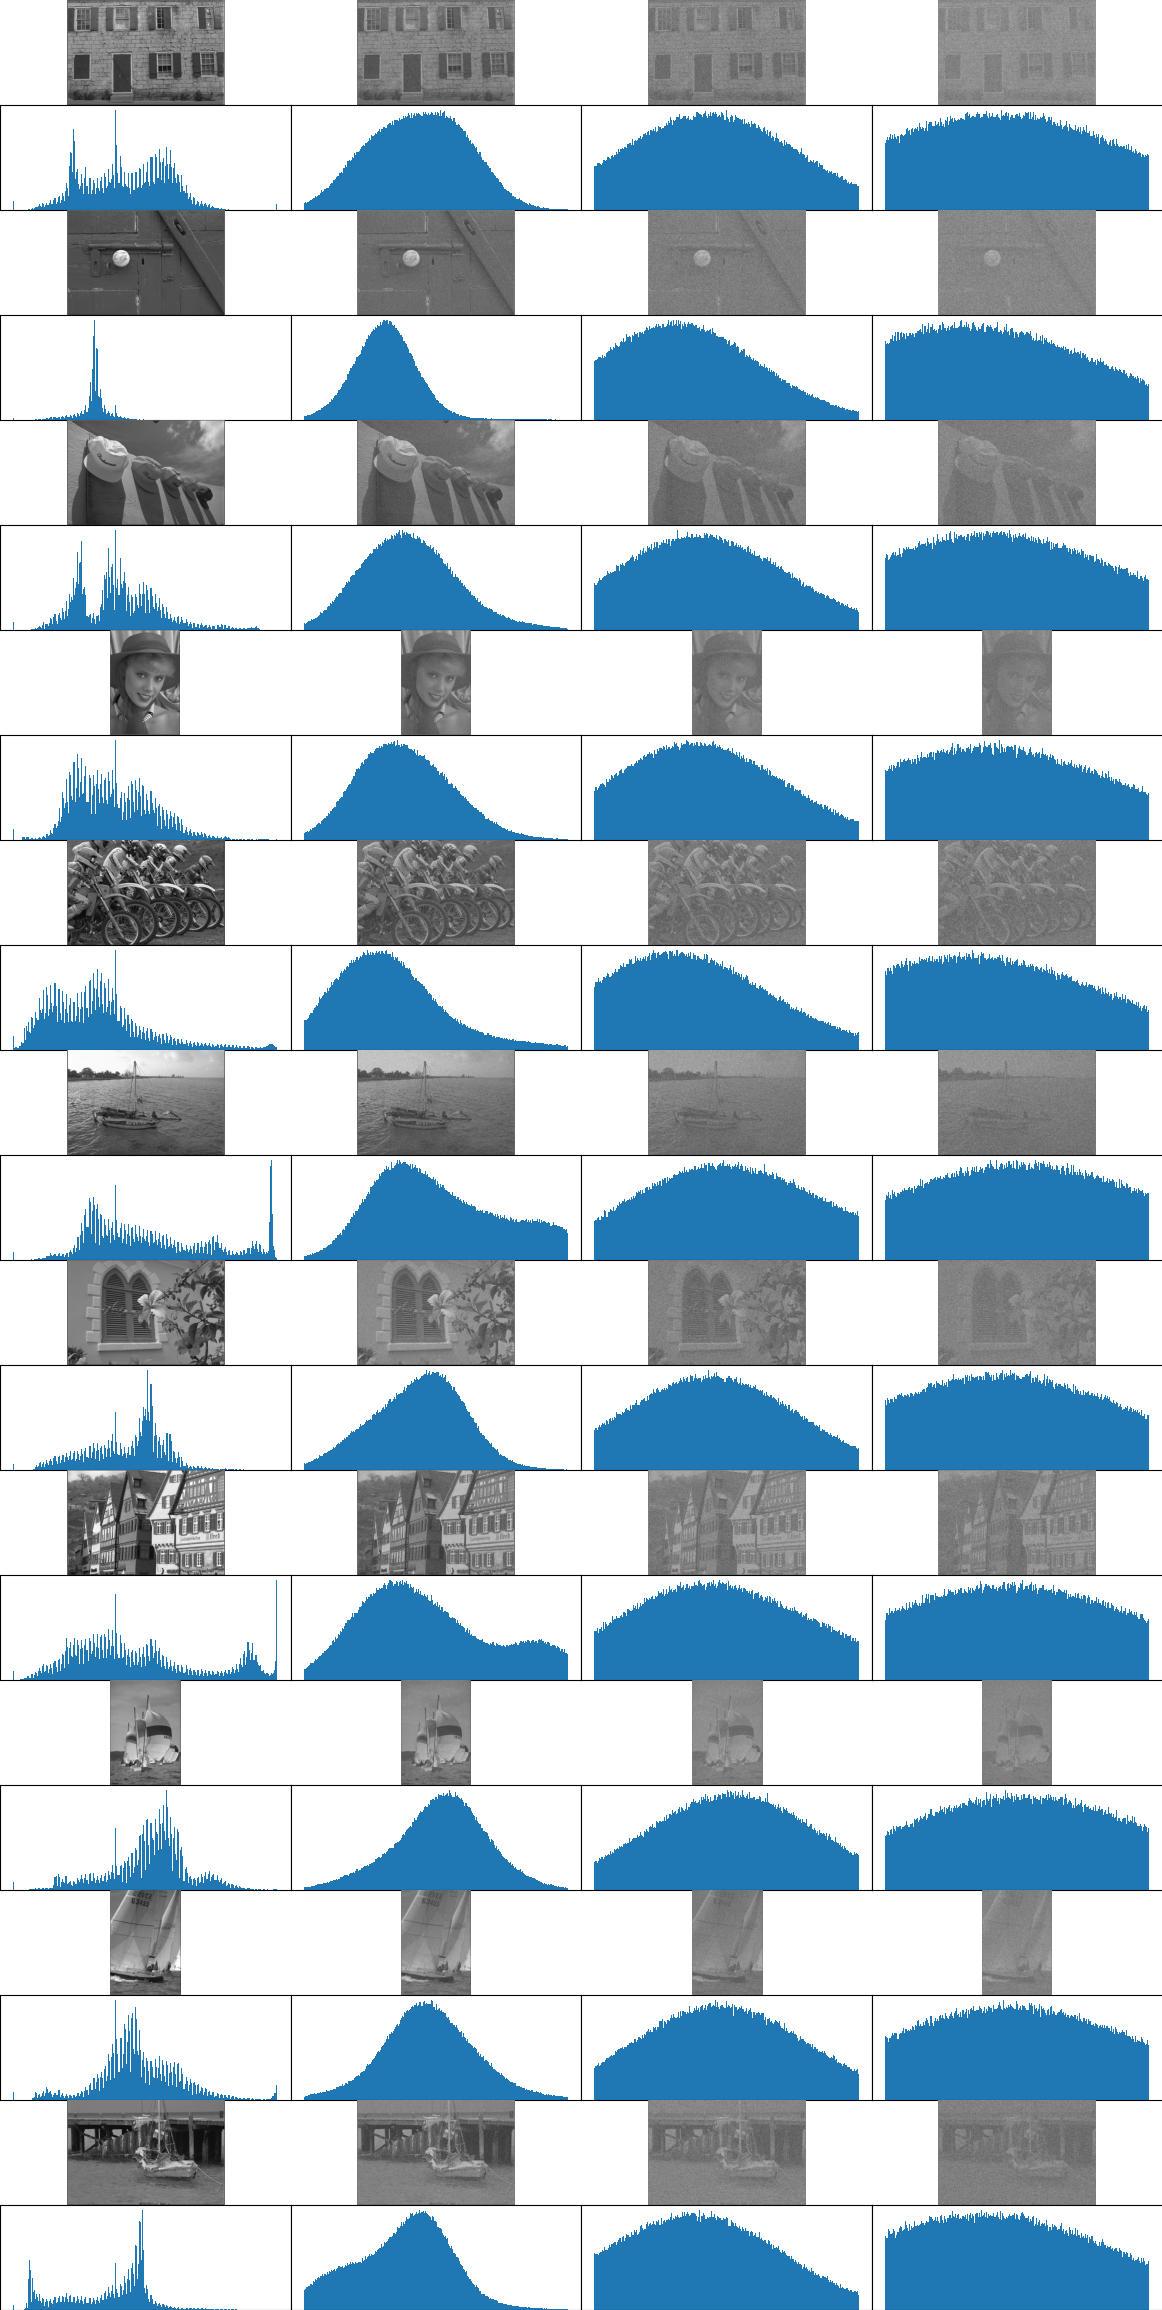
\includegraphics[width=0.6\textwidth]{figuras/img_hist_noise_1.png}
    \caption{Imagen original junto con su histograma con distintos niveles de ruido, primera mitad del banco.}
\end{figure}

\begin{figure}
    \centering
    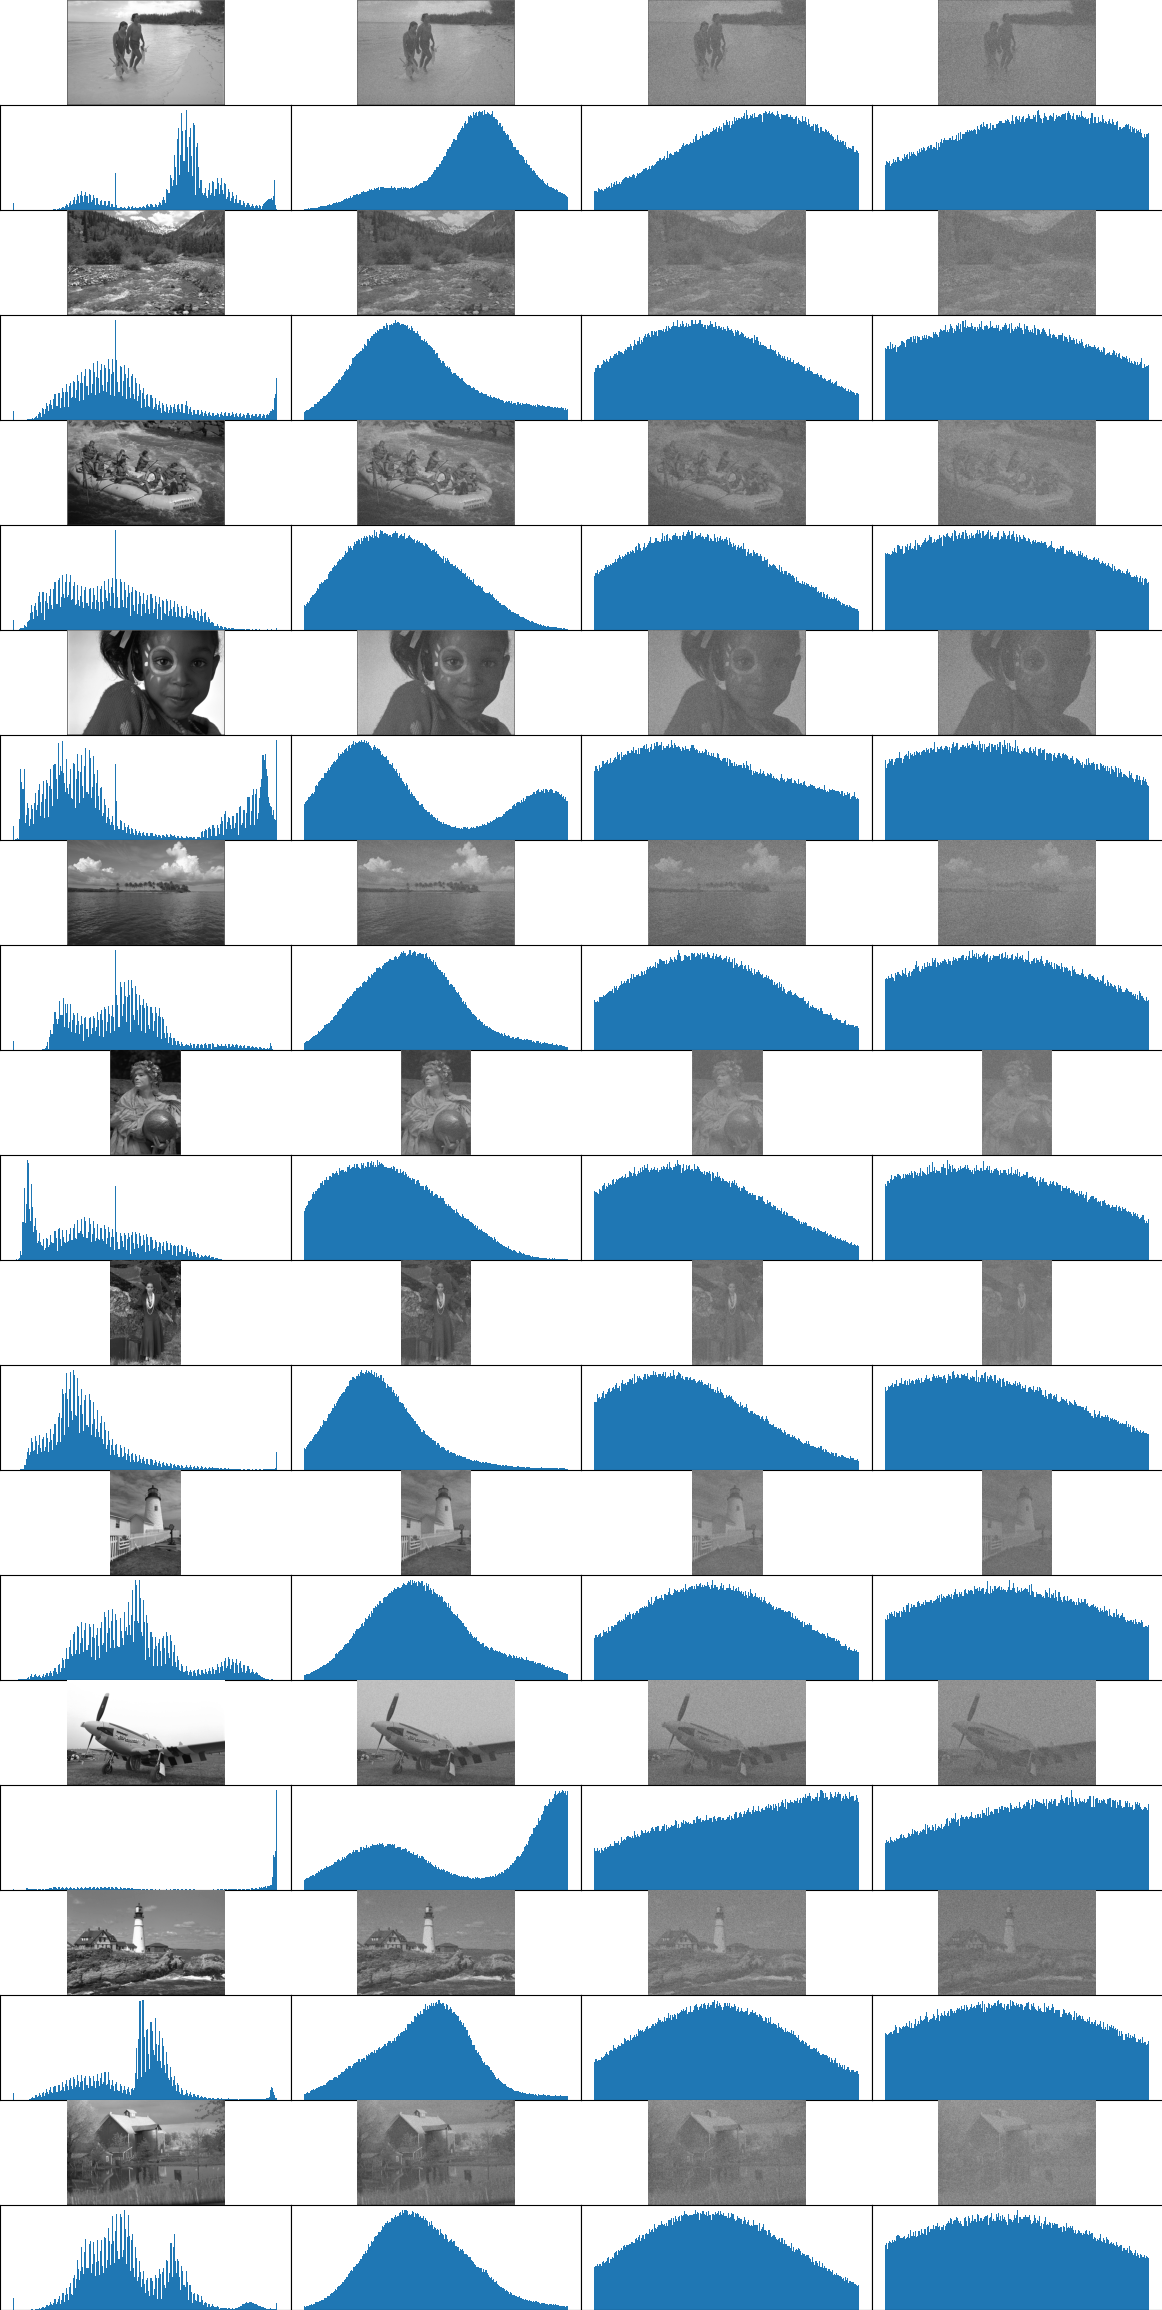
\includegraphics[width=0.6\textwidth]{figuras/img_hist_noise_2.png}
    \caption{Imagen original junto con su histograma con distintos niveles de ruido, segunda mitad del banco.}
\end{figure}


\begin{figure}
    \centering
    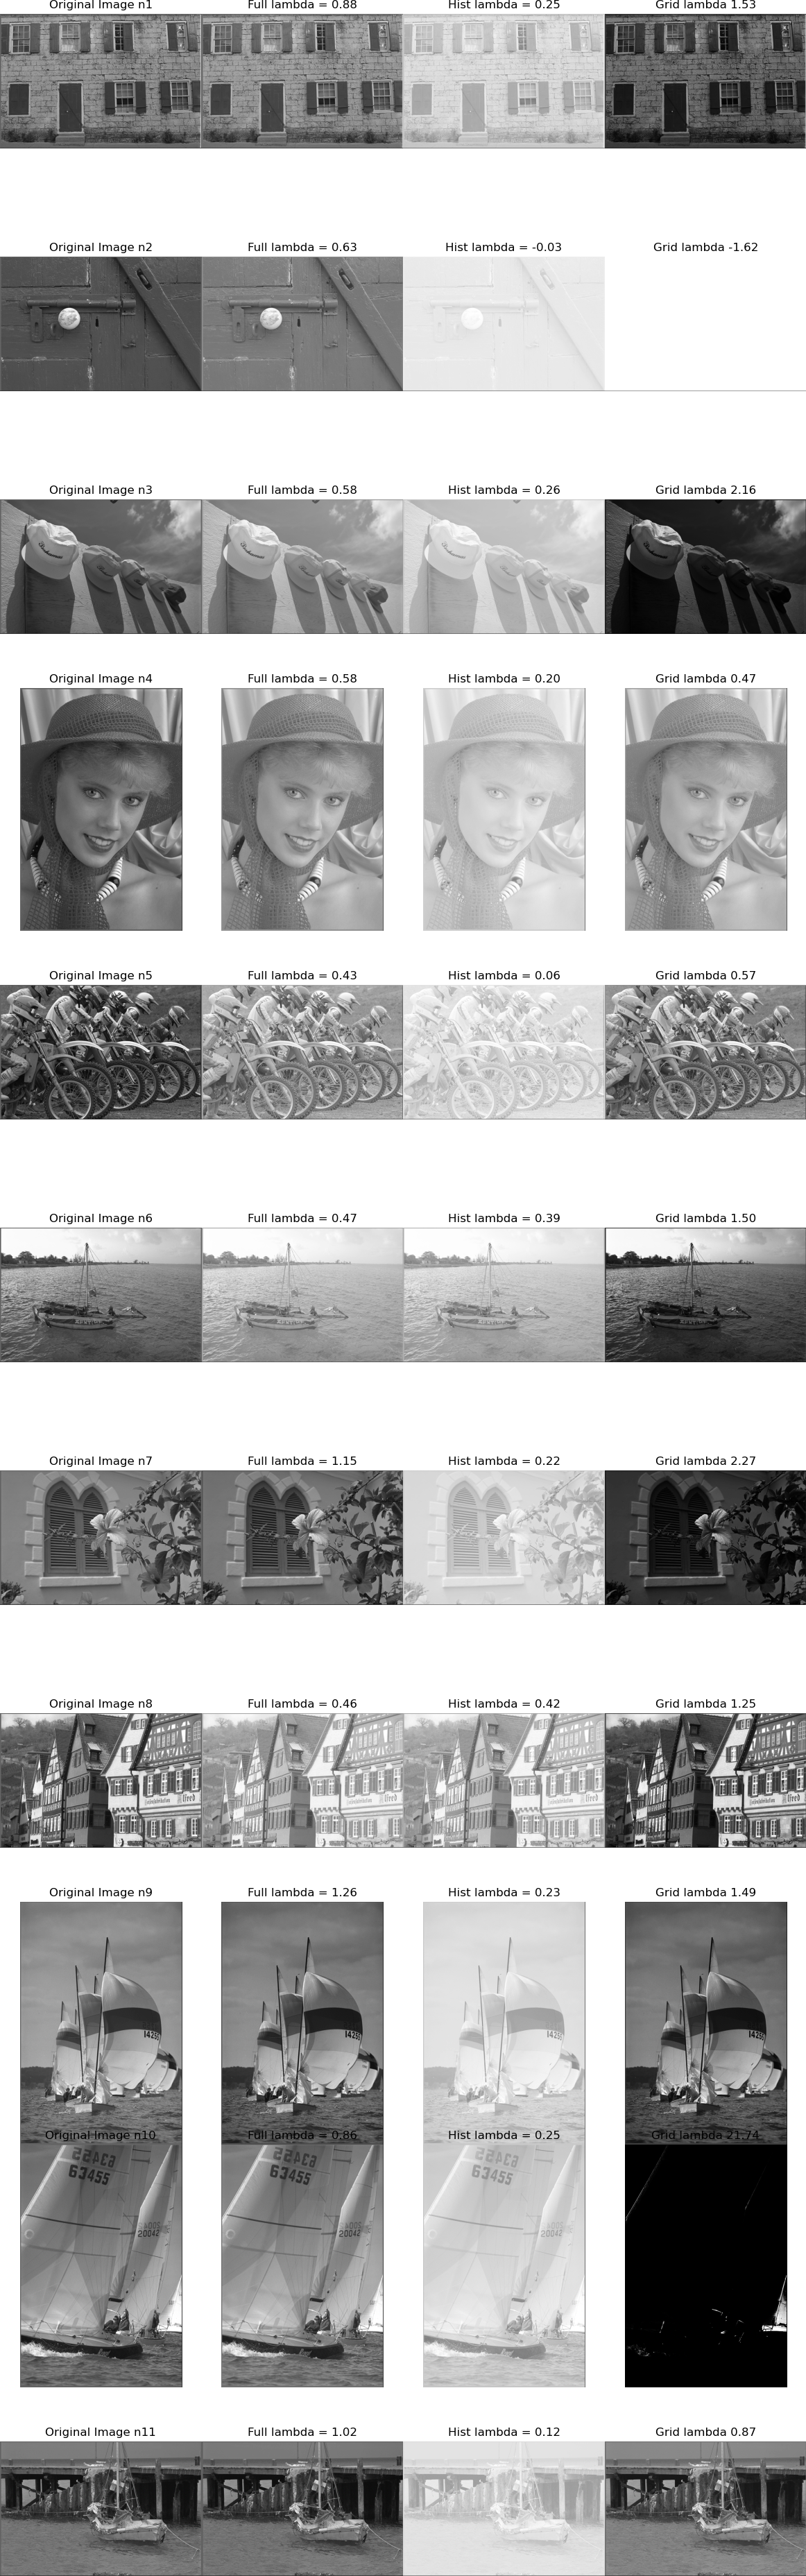
\includegraphics[width=0.4\textwidth]{figuras/img_BCI_all_1.png}
    \caption{Imagen original junto con sus transformaci\'ones Box-Cox para los distintos m\'etodos de lambda transformados, primera mitad del banco.}
\end{figure}

\begin{figure}
    \centering
    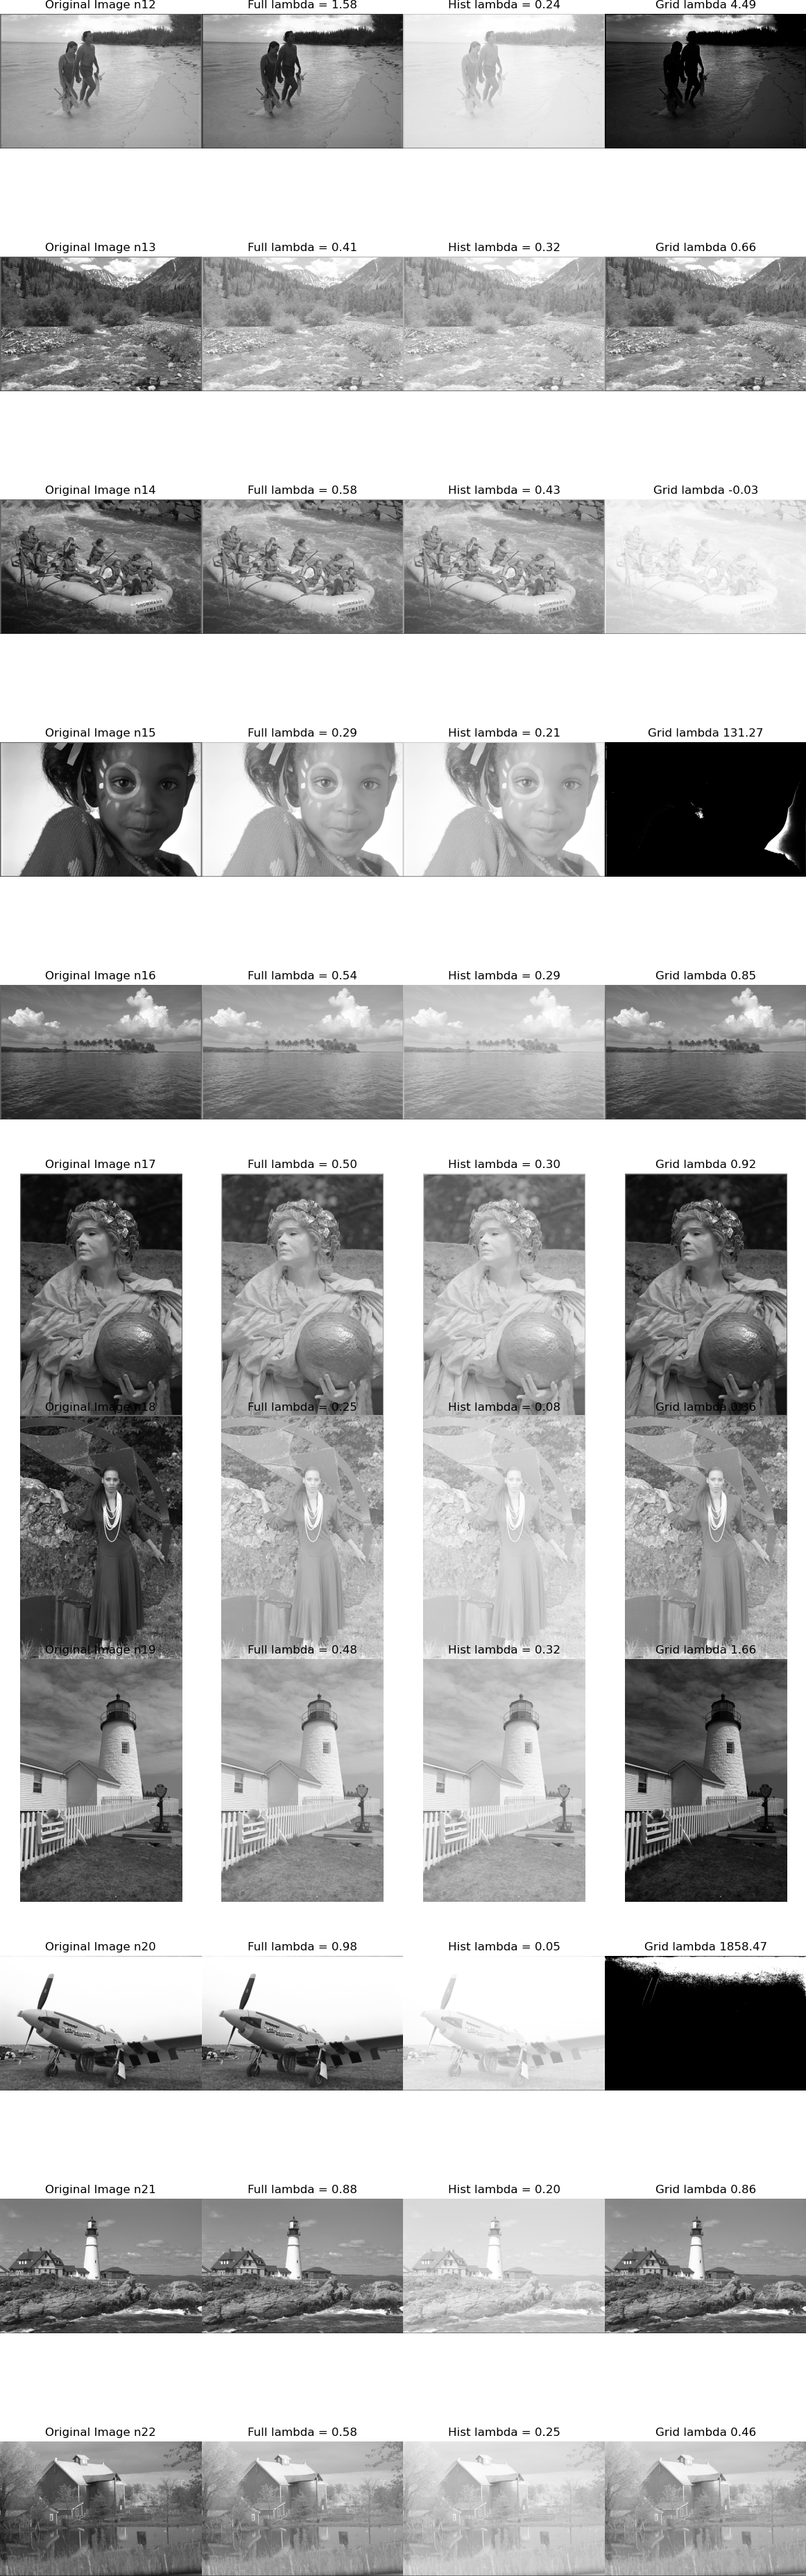
\includegraphics[width=0.4\textwidth]{figuras/img_BCI_all_2.png}
    \caption{Imagen original junto con sus transformaci\'ones Box-Cox para los distintos m\'etodos de lambda transformados, segunda mitad del banco.}
\end{figure}

\begin{figure}
    \centering
    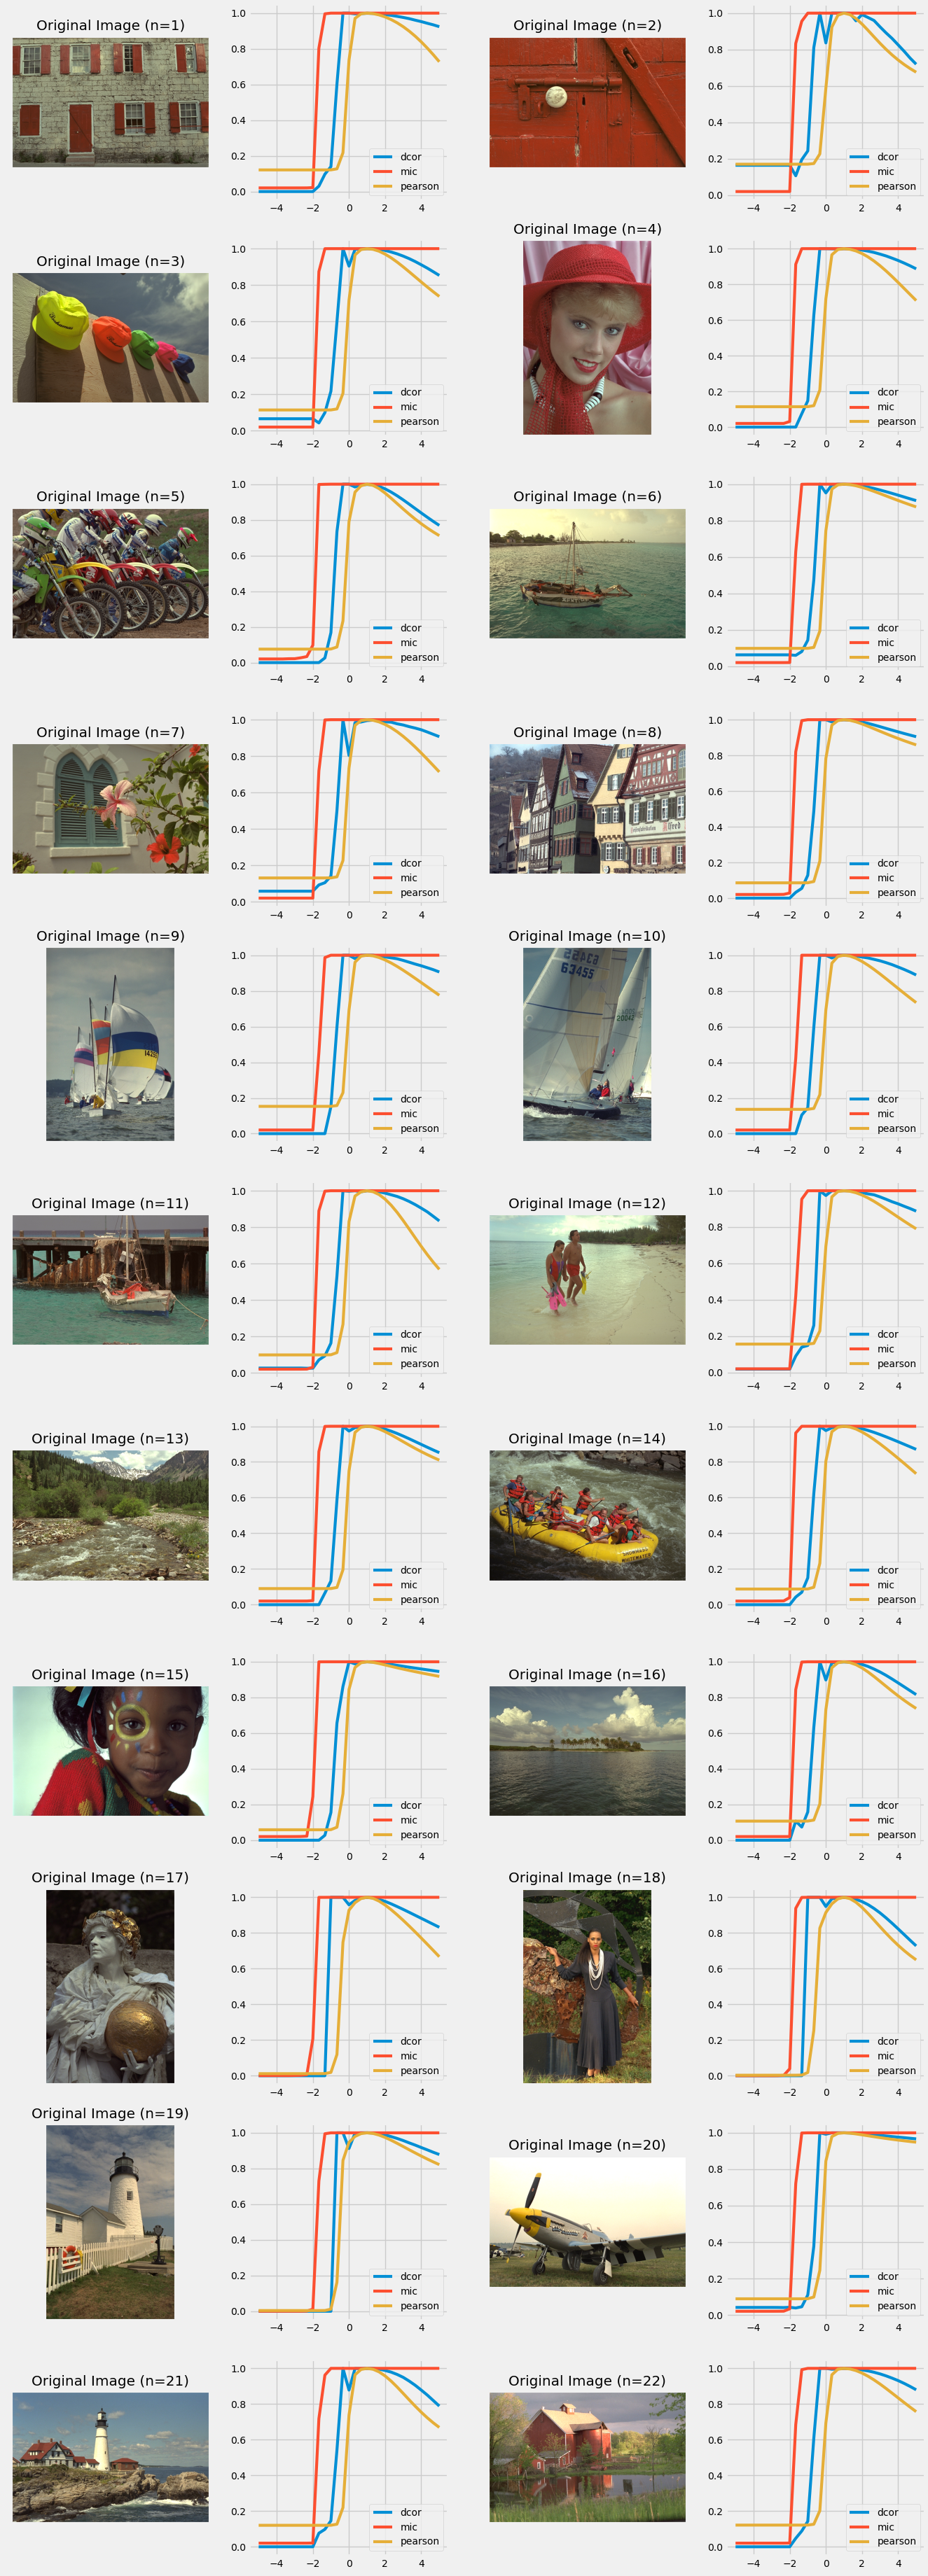
\includegraphics[width=0.5\textwidth]{figuras/full_comp.png}
    \caption{A la izquierda la im\'agen original y a la derecha el valor de $dCor$ (azul), $MIC$ (rojo), y $\rho$ (amarillo) utilizando el vector completo en el eje y, $\lambda$ en el eje x.}
\end{figure}

\begin{figure}
    \centering
    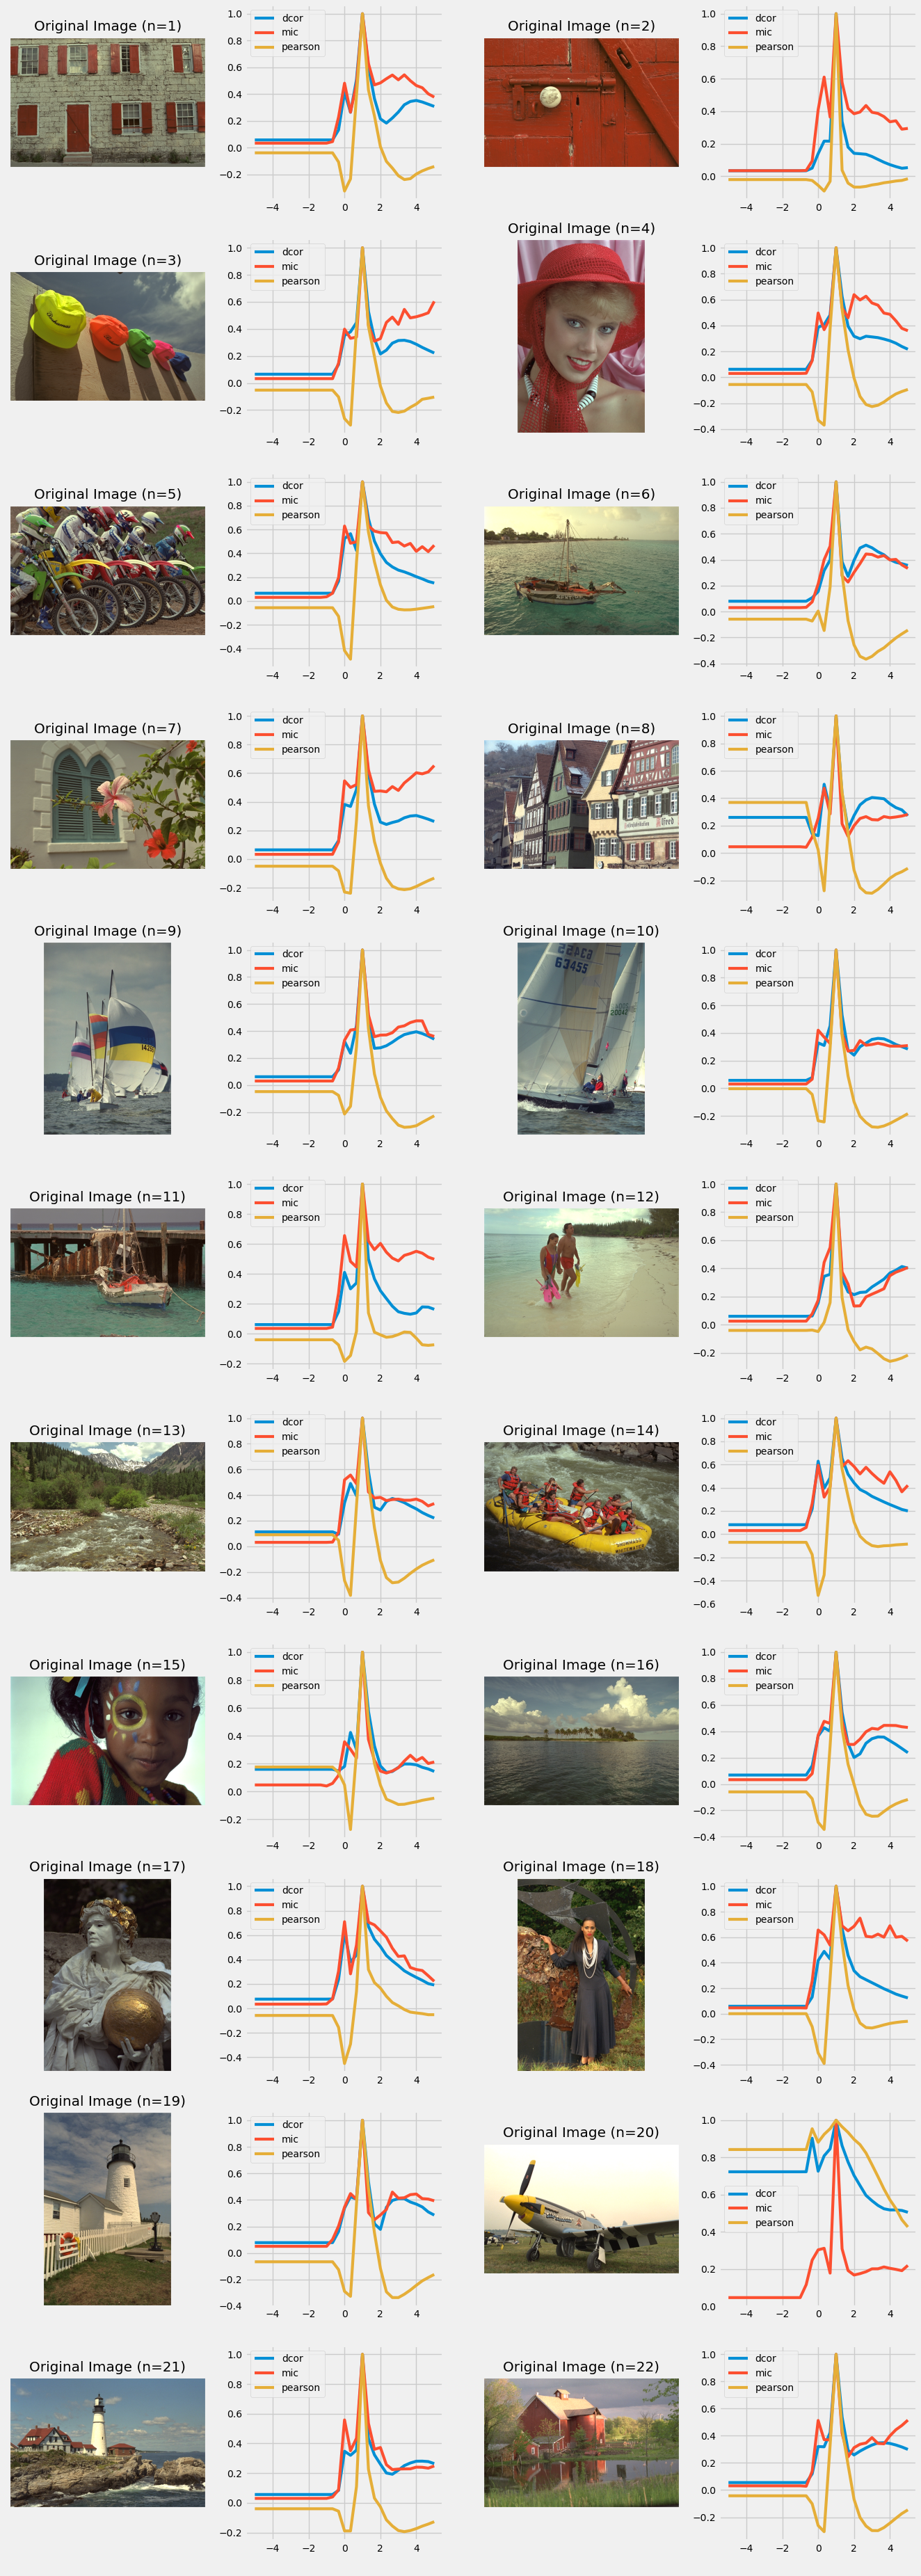
\includegraphics[width=0.5\textwidth]{figuras/hist_comp.png}
    \caption{A la izquierda la im\'agen original y a la derecha el valor de $dCor$ (azul), $MIC$ (rojo), y $\rho$ (amarillo) utilizando el histograma en el eje y, $\lambda$ en el eje x.}
\end{figure}

% ---------------------------------------------------------------------------------------------